\documentclass[11pt, oneside]{article}   	% use "amsart" instead of "article" for AMSLaTeX format
\usepackage{geometry}                		% See geometry.pdf to learn the layout options. There are lots.
\geometry{letterpaper}                   		% ... or a4paper or a5paper or ... 
%\geometry{landscape}                		% Activate for for rotated page geometry
%\usepackage[parfill]{parskip}    		% Activate to begin paragraphs with an empty line rather than an indent
\usepackage{graphicx}				% Use pdf, png, jpg, or eps� with pdflatex; use eps in DVI mode
								% TeX will automatically convert eps --> pdf in pdflatex		
\usepackage{amssymb}
\usepackage{amsmath}
\usepackage{parskip}
\usepackage{color}
\usepackage{hyperref}

\title{scratch}
%\author{The Author}
%\section{}
%\subsection*{}
\date{}							% Activate to display a given date or no date

\graphicspath{{/Users/telliott_admin/Dropbox/Tex/png/}}
% \begin{center} 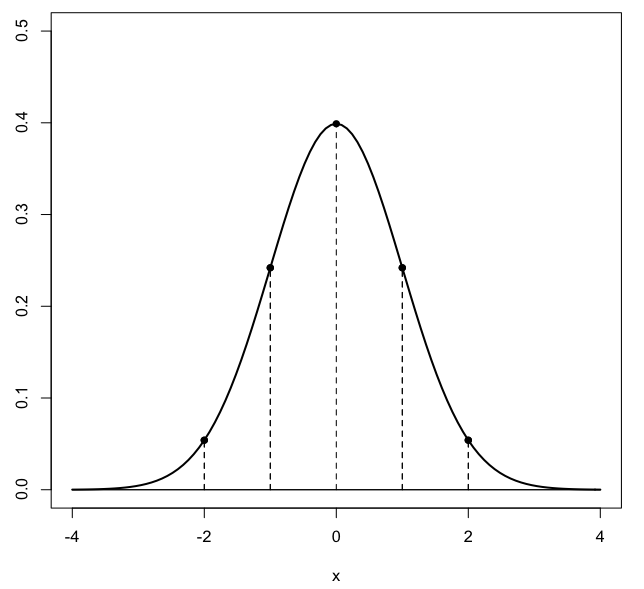
\includegraphics [scale=0.4] {gauss3.png} \end{center}
\begin{document}
\maketitle
\Large
\subsection*{example}
\url{https://www.youtube.com/watch?v=1m70lAiEz0Y}

Find the power series expansion for the following function about the given point $c$, valid for the given region $R$
\[ f(z) = \frac{1}{(z+1)(z+3)}, \ \ \ c = 1 \]
\[ R = \{ z: 2 < |z-1| < 4 \} \]
We're expanding around $c=1$ (i.e. ($1 + 0i$)).  We're working with an annulus of inner radius $2$ and outer radius $4$, which include the two singularities at $z = -1$ and $z = -3$.

We expand the function using partial fractions
\[ \frac{1}{(z+1)(z+3)} = \frac{A}{z+1} + \frac{B}{z+3} \]
We have for the numerator that
\[ Az + 3A + Bz + B = 1 \]
so $A = -B$ and then $-2B = 1$ so $B = -1/2$ and $A = 1/2$ and:
\[ f(z) = \frac{1}{2} \ [ \ \frac{1}{z+1} - \frac{1}{z+3} \ ]  \]
and now, according to the video, we are looking for a Laurent series for the first one and a Taylor series for the second one (we're inside the singularity).

For the Taylor series (around the point $1$):
\[ \frac{1}{z + 3} = \frac{1}{(z-1) + 4} = \frac{1}{4} \ \frac{1}{1 + \frac{(z-1)}{4}} \]
\[ = \frac{1}{4} \sum_{n=0}^{\infty} \frac{(-1)^n (z-1)^n}{4^n}, \ \ \ \text{for} \ z - 1 < 4 \]
So where does this come from?  Recall that the geometric series is the Taylor series for $1/1-x$ since
\[ \frac{1}{1-x} = 1 + x + x^2 + x^3 + \dots \]
We can see that this is correct by multiplying out.  Or, we can take the derivatives:
\[ f'(x) = \frac{1}{(1-x)^2} \]
\[ f''(x) = \frac{2}{(1-x)^3} \]
\[ f'''(x) = \frac{3!}{(1-x)^4} \]
The terms (evaluated at $a=0$) are 
\[ \frac{1}{n!} f^n(a)(x-a)^n = x^n \]
For our series we must substitute $-x = x$
\[ \frac{1}{1+x} = 1 - x + x^2 - x^3 + \dots \]
which accounts for the $(-1)^n$ term.  The rest can be obtained by rescaling the variable.

For the Laurent series (around the point $1$):


\end{document}  